In this chapter, we apply MCMC algorithm to learn synchronous graph grammars for mapping strings
to graphs structure. Specifically, we learn Synchronous Hyperedge Replacement Grammar (SHRG) rules from a forest that represents likely derivations consistent with a fixed string-to-graph 
alignment. We make an analogy of string-to-AMR parsing to the task of phrase-based machine translation and
come up with an efficient algorithm to learn graph grammars from string-graph pairs. We propose an effective
approximation strategy to resolve the complexity issue of graph compositions. We also show some useful strategies
to overcome existing problems in an SHRG-based parser and present preliminary results of a graph-grammar-based approach. 
%\section{Introduction} 
%Abstract Meaning Representation (AMR) \cite{banarescu2013abstract} is a semantic formalism where the meaning 
%of a sentence is encoded as a rooted, directed graph. 
%Figure~\ref{fig:amr-example} shows an example of the edge-labeled representation of an AMR 
%graph where the edges are labeled while the nodes are not. The label of the leaf edge going out of a node represents 
%the concept of the node, and the label of a non-leaf edge shows the relation between the concepts of the two nodes it connects to. 
%This formalism is based on propositional logic and neo-Davidsonian event representations~\cite{parsons1990events,Davidson:1967}.
%AMR does not encode quantifiers, tense and modality, but it jointly encodes a set of selected semantic phenomena which renders
%it useful in applications like question answering and semantics-based machine translation.
%
%\begin{figure}
%\begin{center}
%\scalebox{0.50}{
%    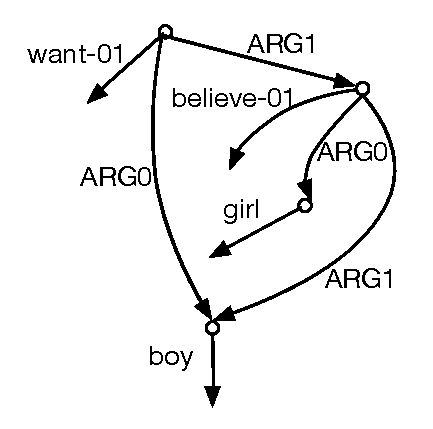
\includegraphics{./amr_example.eps}
%}
%\caption{An example of AMR graph representing the meaning of: ``The boy wants the girl to believe him"}
%\label{fig:amr-example}
%\vspace{-1em}
%\end{center}
%\end{figure}
%The task of AMR graph parsing 
%is to map natural language strings to AMR semantic graphs. \namecite{flanigan2014discriminative} propose a two-stage parsing
%algorithm which first maps meaningful continuous spans on the string side to concept fragments
%on the graph side, and then in the second stage adds additional edges to
%make all these fragments connected. Concept identification \cite{flanigan2014discriminative,pourdamghanialigning} can be considered as an important first step to
%relate components of the string to components in the graph.
%
%
%\namecite{wang-xue-pradhan:2015:NAACL-HLT} also present a two-stage procedure where they first use a dependency parser
%trained on a large corpus to generate a dependency tree for each sentence. In the second step, a transition-based algorithm
%is used to greedily modify the dependency tree into an AMR graph. The 
%benefit of starting with a dependency tree instead of the original sentence is that the dependency structure is 
%more linguistically similar to an AMR graph and provides more direct feature information within limited
%context.
%
%
%Hyperedge replacement grammar (HRG) is a context-free rewriting formalism for generating graphs~\cite{drewes+al:1997}. 
%Its synchronous counterpart, SHRG, can be used for transforming a graph from/to another structured representation such as a string
%or tree structure. HRG has great potential for applications in natural language understanding and generation,
%and also semantics-based machine translation. 
%
%
%Given a graph as input, finding its derivation of HRG rules is NP-complete~\cite{drewes+al:1997}. 
%\namecite{chiang-acl13} describe in detail a graph recognition algorithm
%and present an optimization scheme which enables the
%parsing algorithm to run in polynomial time when the treewidth and degree
%of the graph are bounded. However, there is still no real system available
%for parsing large graphs.
%
%
%An SHRG can be used for AMR graph parsing where each SHRG rule consists of a pair of a CFG rule and an HRG rule, 
%which can generate strings and AMR graphs in parallel. 
%\namecite{jones2012semantics} present a Syntactic Semantic Algorithm that learns SHRG by matching minimal parse constituents
%to aligned graph fragments and incrementally collapses them into hyperedge nonterminals. 
%The basic idea is to use the string-to-graph alignment and syntax information to constrain the possible HRGs.
%
%
%Learning SHRG rules 
%from fixed string-to-graph alignments is a similar problem to extracting machine translation rules from fixed word
%alignments, where we wish to automatically learn the best granularity for the rules with which to analyze each
%sentence. \namecite{chung-cl14} present an MCMC sampling schedule to learn Hiero-style SCFG rules \cite{ChiangCL} by sampling 
%tree fragments from phrase decomposition forests, which represent all possible
%rules that are consistent with a set of fixed word alignments, making use of the property that each SCFG rule in the 
%derivation is in essence the 
%decomposition of a larger phrase pair into smaller ones.
%
%
%In this paper, we make an analogy to treat fragments in the graph language as phrases in the natural language string 
%and SHRG rules as
%decompositions of larger substring, graph fragment pairs into smaller ones. 
%Graph language is different
%from string language in that there is no explicit order to compose the graph and there is an exponential number of possible 
%compositions. We propose a strategy that uses the left-to-right order of the string to constrain the structure of the 
%derivation forest and experiment with different tactics in dealing with unaligned words on the string side and unaligned
%edges on the graph side.
%
%
%\section{Hyperedge Replacement Grammar}
%\begin{figure}
%\begin{center}
%\resizebox{\linewidth}{!}{
%\scalebox{0.45}{
%    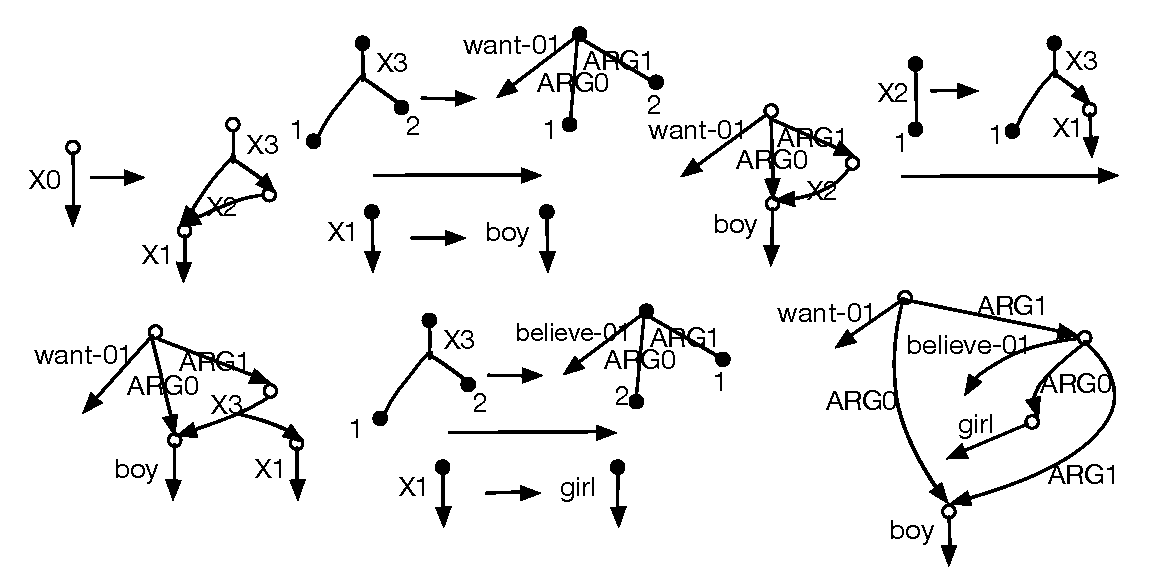
\includegraphics{./HRG.eps}
%}
%}
%\caption{The series of HRG rules applied to derive the AMR graph of ``The boy wants the girl to believe him". The first rule is directly shown. The other HRG rules
%are either above or below each right arrow. The white circle shows the root of each hyperedge. The indexes in each rule show the one-to-one mapping
%between the attachment nodes of l.h.s.\ nonterminal edges and the external nodes of the r.h.s.\ subgraph}
%\label{fig:hrg-example}
%\vspace{-1em}
%\end{center}
%\end{figure}
%Hyperedge replacement grammar (HRG) is a context-free rewriting formalism for graph generation \cite{drewes+al:1997}. 
%HRG is like CFG in that it rewrites nonterminals independently.
%While CFG generates natural language strings by successively rewriting nonterminal tokens, the nonterminals in 
%HRG are hyperedges, and each rewriting step in HRG replaces a hyperedge nonterminal with a subgraph instead of a span of a string.
%\subsection{Definitions}
%In this paper we only use edge-labeled graphs
%because using both node and edge labels complicates the definitions in our HRG-based approach. Figure~\ref{fig:hrg-example} 
%shows a series of HRG rules applied to derive the AMR graph shown in Figure~\ref{fig:amr-example}.
%
%
%We start with the definition of hypergraphs. An {\em edge-labeled, directed hypergraph} is a tuple $H=\langle V,E,l,X\rangle$, where $V$ is a finite set of nodes, $E\subseteq V^+$ is
%a finite set of hyperedges, each of which will connect to one or more nodes in $V$. $l: E\to L$ defines a mapping from each 
%hyperedge to its label from a finite set $L$. Each hyperedge is an atomic item with an ordered list of nodes it connects to, which 
%are called attachment nodes. The {\em type} of a hyperedge
%is defined as the number of its attachment nodes.  $X\in V^*$ defines an ordered list of distinct nodes called
%{\em external nodes}. 
%The ordered external nodes specify how to fuse a
%hypergraph with another graph, as we will see below.
%In this paper, we alternately use the terms of 
%hypergraph and graph, hyperedge and edge, and also phrase, substring and span for brevity.
%
%
%An HRG is a rewriting formalism $G=\langle N,T,P,S \rangle$, where $N$ and $T$ define two disjoint finite sets called nonterminals 
%and terminals. $S\in N$ is a special nonterminal
%called the start symbol. $P$ is a finite set of productions of the form $A\to R$, where $A\in N$ and $R$ is a 
%hypergraph with edge labels over $N\cup T$ and with nonempty external nodes $X_R$. We have the constraint that the type of the
%hyperedge with label $A$ should coincide with the number of nodes in $X_R$. In our grammar, each nonterminal
%has the form of $Xn$, where $n$ indicates the type of the hyperedge. Our special start symbol is separately denoted as $X0$.
%
%
%The rewriting mechanism replaces a nonterminal 
%hyperedge with the graph fragment specified by a production's
%righthand side (r.h.s),\ attaching each external node of the 
%r.h.s.\ to the corresponding attachment node of the lefthand side.
%Take Figure~\ref{fig:hrg-example} as an example. 
%Starting from our initial hypergraph with one edge 
%labeled with the start symbol $``X0"$, we select one edge with nonterminal label in our current hypergraph, 
%and rewrite it using a rule in our HRG\@. The first rule rewrites
%the start symbol with a subgraph shown on the r.h.s..\ We continue the rewriting steps 
%until there are no more nonterminal-labeled edges. 
%
%
%The synchronous counterpart of HRG can be used for transforming graphs from/to another form of natural language representation. 
%Productions have the form $(A\to \langle S, R\rangle , \sim)$, where $A \in N$ and $S$ and $R$ are called the source and the target and at least one of them should be
%hypergraphs over $N\cup T$. $\sim$ is a bijection linking nonterminals mentions in $S$ and $R$.
%In our case, the source side is a CFG and the target side is an HRG\@. Given such a synchronous grammar and a string as input, we can 
%parse the string with the CFG side and then derive the counterpart graph by deduction from the derivation. The benefit of 
%parsing with SHRG is that the complexity is bounded by a CFG-like parsing.
%
%\subsection{SHRG-based AMR graph parsing}
%\begin{figure}
%\begin{center}
%\resizebox{\linewidth}{!}{
%\scalebox{0.45}{
%    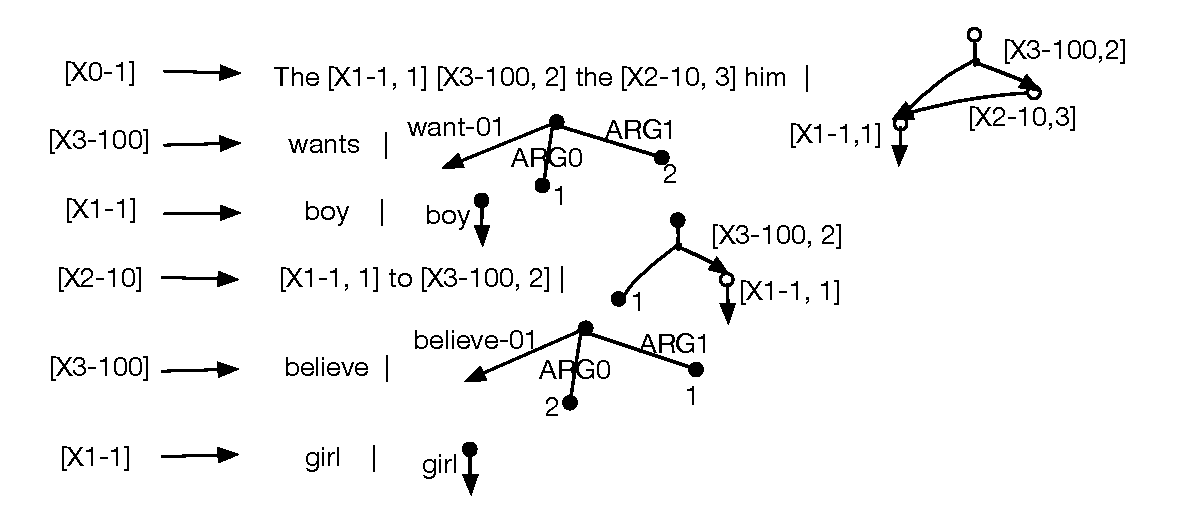
\includegraphics{./SHRGrules.eps}
%}
%}
%\caption{A series of symbol-refined SHRG rules used to derive the AMR graph for the sentence ``The boy wants the girl to believe him".}
%\label{fig:shrg-example}
%\vspace{-1em}
%\end{center}
%\end{figure}
%We write down AMR graphs as rooted, directed, edge-labeled graphs. There is exactly one leaf edge 
%going out of each node, the label of which represents the concept of the node. We define
%this leaf edge as {\bf concept edge}. In Figure~\ref{fig:amr-example}, for example, the edge labeled 
%with ``boy", ``want-01", ``girl" or ``believe-01" connects to only one node in the AMR graph and
%each label represents the concept of that node.
%AMR concepts are either English words (``boy"), PropBank framesets (``want-01"), or special keywords like
%special entity types, quantities, and logical conjunctions. The label of each non-leaf edge shows the relation
%between the AMR concepts of the two nodes it connects to. %In the rest of the paper we will use ``want" and ``believe" instead of they frameset representation for brevity.
%
%
%The constraint of having exactly one concept edge for each node 
%is not guaranteed in general SHRG\@. Our strategy for maintaining the AMR graph structure is to refine the 
%edge nonterminal label with an extra binary
%flag, representing whether it will have a concept edge in the
%final rewriting result, for each external node. The basic intuition is to explicitly enforce the one concept edge constraint
%in each nonterminal so that no additional concept edge is introduced after applying each rule. The graph
%derived from this type of SHRG is guaranteed to have exactly one concept edge at each node.
%
%
%Figure~\ref{fig:shrg-example} shows one example of our symbol-refined SHRG\@.
%For each nonterminal $Xi$-$b_1\cdots b_i$, $i$ defines the type of the nonterminal, while
%each $b_i$ indicates whether the $i$-th external node will have a concept edge
%in the rewriting result.\footnote{$X0$-1 is different as $X0$ is the start symbol of type one and should always have a concept edge at the root}
%%For each $[Xi$-$b_1\cdots b_i, j]$, $i$ defines the type of the nonterminal, while
%%each $b_i$ indicates whether the $i$-th external node will have a concept edge
%%in the rewriting result.\footnote{$X0$-1 is different as $X0$ is the start symbol of type one and should always have a concept edge at the root} 
%%$j$ indicates the one to one mapping from the nonterminals
%%on the string side to the nonterminal edges on the graph side.
%The second rule, for example, rewrites nonterminal $X3$-100 with {\em wants} on the string side and a hypergraph with three external nodes where 
%the root has a concept edge {\em :want-01} as the first binary flag 1 indicates, while the other two external nodes do not with the binary flag 0. 
%This guarantees that when we integrate the r.h.s.\ into
%another graph, it will introduce the concept edge {\em :want-01} to the first fusing position
%and no concept edge to the next two.
%
%
%While this refinement might result in an exponential number of nonterminals with respect to the maximum type of hyperedges, 
%we found in our experiment that most of the nonterminals
%do not appear in our grammar. We use a maximum edge type of 5, which also results in a relatively small nonterminal set.
%\section{Sampling SHRG from forests}
%The fragment decomposition forest provides a compact representation of all possible SHRG rules that are consistent with a fixed string-to-graph 
%alignment. Each SHRG rule in the derivation is in essence the decomposition of 
%larger phrase, graph fragment pairs on the left hand side (l.h.s.)\ into smaller ones on the r.h.s.\ and is
%encoded in a tree fragment in the forest. Our goal is to learn an SHRG from this forest.
%We first build a forest representation of possible derivations and then use an MCMC algorithm to
%sample tree fragments from this forest representing each rule in the derivation.
%\subsection{Fragment Decomposition Forest}
%We first proceed to define the {\bf fragment decomposition forest}. The fragment decomposition forest is a variation of
%the phrase decomposition forest defined by \namecite{chung-cl14} where the target side is a graph instead of a string.
%
%
%$$\resizebox{.88\hsize}{!}{$\displaystyle
%\overbrace{The}^\text{$\emptyset$}\ \overbrace{boy}^\text{\begin{tikzpicture}\draw (0,0) node[draw,ellipse]{boy}; \end{tikzpicture}}
%\overbrace{wants}^\text{\begin{tikzpicture}\draw (0,0) node[draw,ellipse]{want-01};  \end{tikzpicture}} %{want-01};
%\overbrace{the}^\text{$\emptyset$}
%\overbrace{girl}^\text{\begin{tikzpicture}\draw (0,0) node[draw,ellipse]{girl}; \end{tikzpicture}}
%\overbrace{to}^\text{$\emptyset$}
%\overbrace{believe}^\text{\begin{tikzpicture}\draw (0,0) node[draw,ellipse]{believe-01}; \end{tikzpicture}}
%\overbrace{him}^\text{$\emptyset$}$}
%$$
%A {\bf phrase} $p=[i, j]$ is a set of continuous word indices $\{i,i+1,\ldots ,j-1\}$. A {\bf fragment} $f$ is 
%a hypergraph with external nodes $X_f$. A string-to-graph alignment $h: P \to F$ defines the mapping from
%spans in the sentence to fragments in the graph.
%Our smallest phrase-fragment pairs are the string-to-graph alignments extracted using heuristic
%rules from \namecite{flanigan2014discriminative}.
%The figure above shows an example of the alignments for the sentence ``The boy wants the
%girl to believe him". The symbol $\emptyset$ represents that the word is not aligned to any concept in the AMR graph and this word is called an {\bf unaligned word}. 
%After this alignment, there are also left-over edges that are not aligned from any substrings, which are called
%{\bf unaligned edges}.
%
%
%Given an aligned string, AMR graph pair, 
%a phrase-fragment pair $n$ is a pair $([i, j], f )$ which defines a pair of a phrase $[i,j]$ and a fragment $f$ such
%that words in positions $[i,j]$ are only aligned to concepts in the fragment $f$ and vice versa (with unaligned words and edges omitted).
%%, the definition of which will be clear later
%A fragment forest $H=\langle V, E \rangle$ is a hypergraph made of a set of
%hypernodes $V$ and hyperedges $E$. Each node $n=([i, j], f)$ is {\bf tight} on the string side similar to 
%the definition by \namecite{Koehn-naacl03}, i.e., $n$ contains no unaligned words at its boundaries. 
%Note here we do not have the constraint that $f$ should be connected or single rooted, but we 
%will deal with these constraints separately in the sampling procedure.
%
%
% We define two phrases $[i_1,j_1],[i_2,j_2]$ to be \textit{adjacent} if word indices $\{j_1,j_1+1,\ldots ,
% i_2-1\}$ are all unaligned. We also define two fragments $f_1=\langle V_1, E_1 \rangle, f_2=\langle V_2, E_2\rangle$ to be \textit{disjoint}
%if $E_1 \cap E_2 = \emptyset$. And $f_1$ and $f_2$ are
%adjacent if they are disjoint and $f = \langle V_1 \cup V_2, E_1 \cup E_2\rangle$ is connected.
%We also define the $compose$ operation of two nodes: it takes
%%$n = ([i_1, j_2], f)$ to be the result of $compose$ operation of 
%two nodes $n_1=([i_1, j_1], f_1)$ and $n_2=([i_2, j_2], f_2)$ ($j_1 \leq i_2$) as input, and computes $f = \langle V_1 \cup V_2, E_1 \cup E_2\rangle$,
%the output is a composed node $n=([i_1, j_2], f)$. We say $n_1$ and $n_2$ are \textit{immediately adjacent} if $f$ is connected and single-rooted.
%
%
%\begin{figure}
%\begin{center}
%%\resizebox{\linewidth}{!}{
%\scalebox{0.30}{
%    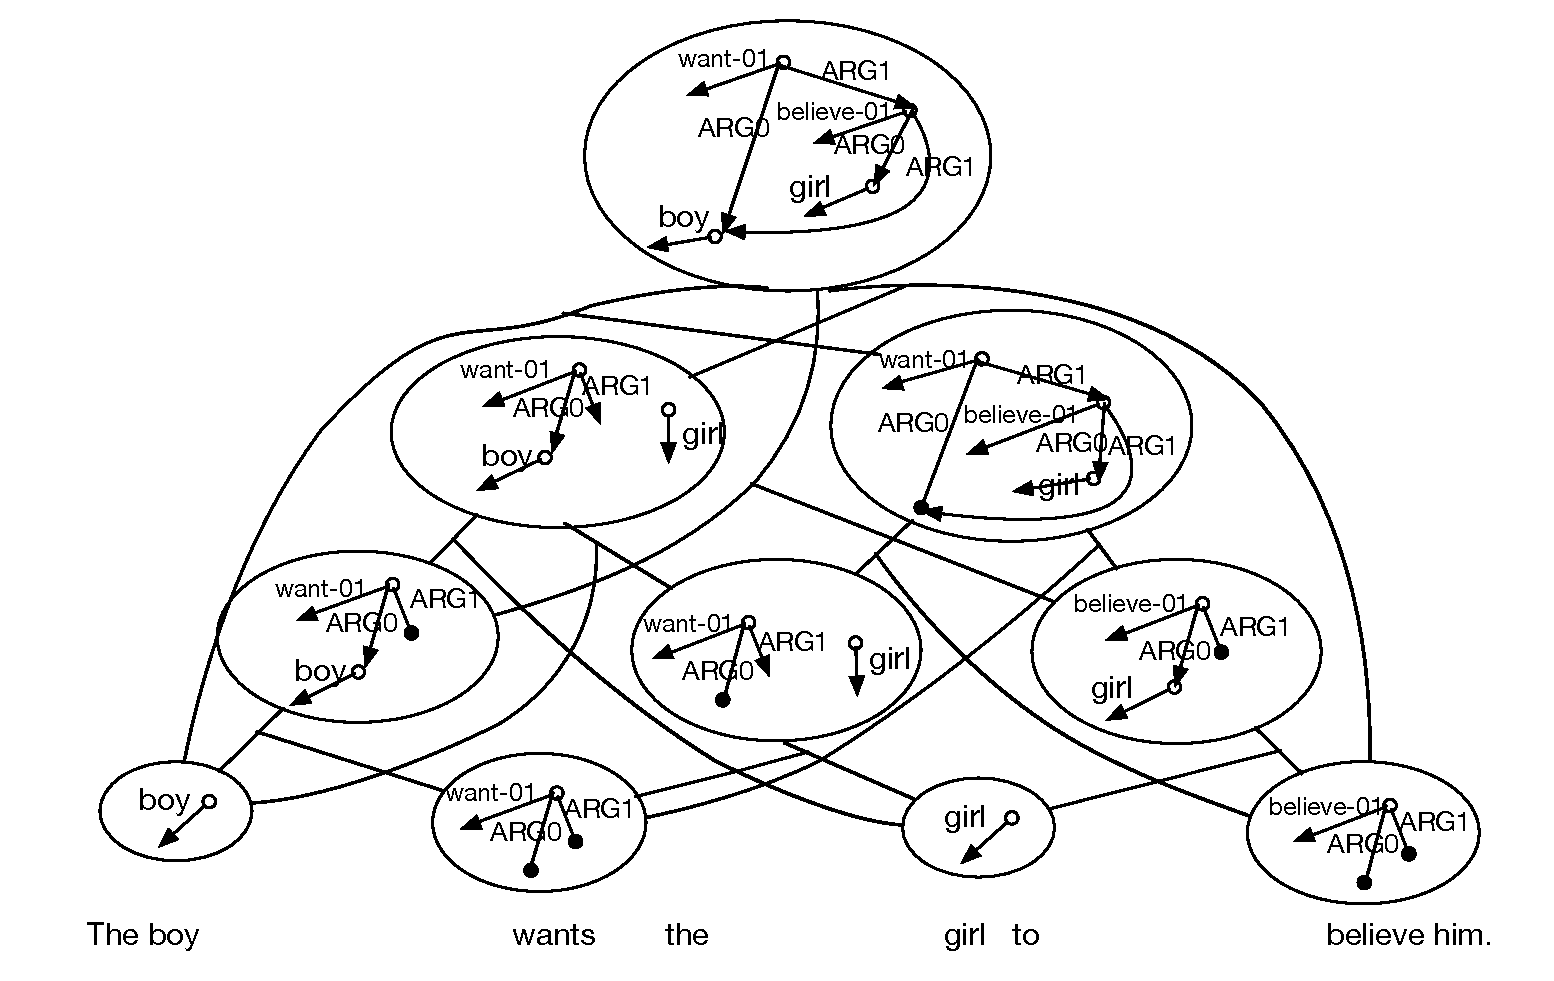
\includegraphics{./HRGForest.eps}
%}
%%}
%\caption{The fragment decomposition forest for the (sentence, AMR graph) pair for ``The boy wants the girl to believe him"}
%\label{fig:decompose-example}
%\vspace{-1em}
%\end{center}
%\end{figure}
%We keep composing larger phrase-fragment pairs (each one kept in a node of the forest) from smaller ones until we reach the root of the forest whose
%phrase side is the whole sentence and the fragment side is the complete AMR graph.
%We define {\bf fragment decomposition forest} to be made of all possible phrase-fragments pairs that can
%be decomposed from the sentence AMR graph pair. The fragment decomposition forest has the important property
%that any SHRG rule consistent with the string-to-graph alignment corresponds to a continuous
%tree fragment of a complete tree found in the forest. 
%
%
%While we can compose larger 
%phrases from smaller ones from left to right, there is no explicit order of composing the graph fragments. Also, the number of possible 
%graph fragments is highly exponential as we need to make a binary decision to decide each boundary node of the fragment and 
%also choose the edges going out of each boundary node of the fragment, unlike the polynomial numbers of phrases for fixed string alignment.
%
%
%Our bottom-up construction procedure starts from the 
%%string-to-graph alignment extracted using \namecite{flanigan2014discriminative}, which are our 
%smallest phrase-fragment pairs.
%We first index these smallest phrase-fragment pairs $([i_k, j_k], f_k), k = 1, 2, \ldots, n$ based on ascending order of their start positions 
%on the string side, i.e., 
%$j_k \leq i_{k+1}$ for $k = 1, 2, \ldots, n-1$. Even with this left-to-right order constraint from the string side, the complexity of
%building the forest is still exponential due to the 
%possible choices in attaching graphs edges that are not aligned to the string. 
%Our strategy
%is to deterministically attach each unaligned relation edge to one of the identified concept 
%fragments it connects to. We attach {\em ARG}s and {\em op}s to its head
%node and each other types of unaligned relations to its tail node.\footnote{Our intuition is that the ARG types for verbs and ops structure
%usually go with the concept of the head node. We assume that other relations are additional introduced to the head node, which resembles
%a simple binarization step for other relations.}
%
%\begin{algorithm}[t]
%\small
%\caption{A CYK-like algorithm for building a fragment decomposition forest}
%\begin{algorithmic}[1]
%    \STATE{For each smallest phrase-fragment pairs $([i_k, j_k], f_k)$, $k$ = $1, 2, \ldots , n$, attach unaligned edges to fragment $f_k$, denoting the result as $f_k'$. Build a node 
%    for $([i_k, j_k], f_k')$ and add it to chart item $c[k][k+1]$.} \label{1st}
%    \STATE{Extract all the remaining unaligned fragments, build a special unaligned node for each of them and add it to unaligned node set $unaligned\_nodes$} \label{2nd}
%    \STATE{Keep composing unaligned nodes with nodes in different chart items if they are immediate adjacent and add it to the same chart item} \label{3rd}
%    \FOR{$span$ from 2 to $n$} \label{4th}
%        \FOR{$i$ from 1 to $n$-$span$+1}
%            \STATE{$j$ = $i$ + $span$}
%            \FOR{$k$ from $i+1$ to $j-1$}
%                \FOR{$n1=([start_1, end_1], f_1)$ in $c[i][k]$}
%                    \FOR{$n2=([start_2, end_2], f_2)$ in $c[k][j]$}
%                        \IF{$f_1$ and $f_2$ are disjoint}
%                        \STATE{$new\_node$ = $compose(n1, n2)$} \label{new}
%                            \STATE{add incoming edge $(n1, n2)$ to $new\_node$}
%                            \IF{$n_1$ and $n_2$ are not {\em immediate adjacent}} \label{5th}
%                                \STATE{$new\_node.nosample\_cut$=True}
%                                \ENDIF \label{6th}
%                                \STATE{{\em insert\_node}($new\_node$, $c[i][j]$)} \label{7th}
%                        \ENDIF
%                    \ENDFOR
%                \ENDFOR
%            \ENDFOR
%        \ENDFOR
%    \ENDFOR
%  \end{algorithmic} 
%  \label{alg:forest} 
%\end{algorithm}
%Algorithm~\ref{alg:forest} shows our CYK-like forest construction algorithm. We maintain the length 1 chart items according to the order of each smallest phrase-fragment
%pair instead of its position in the string.\footnote{We use this strategy mainly because the alignments available do not have
%overlapping alignments, while our algorithm could still be easily adapted to a version that maintains the chart items with string
%positions when overlapping alignments are available} In line~\ref{1st}, we first attach unaligned edges to the smallest phrase-fragment pairs as stated before.
%After this procedure, we build a node for the $k$-th phrase-fragment (with unaligned edges added) pair and add it to chart item $c[k][k+1]$.
%Note here that we still have remaining unaligned edges; in line~\ref{2nd} we attach all unaligned edges going out from the same node as a single fragment and build a special 
%{\bf unaligned node} with empty phrase side and add it to $unaligned\_nodes$ set. In line~\ref{3rd}, we try to compose each unaligned node with one of the nodes in the length 1 chart items
%$c[k][k+1]$. If they are immediately adjacent, we add the composed node to $c[k][k+1]$. 
%The algorithm then composes smaller phrase-fragment pairs into larger ones (line~\ref{4th}). When we have composed two nodes $n_1, n_2$, we need to keep track of this
%incoming edge. We have the constraint in our grammar that the r.h.s.\ hypergraph of each rule
%should be connected and single rooted.\footnote{We should be able to get rid of both constraints as we are parsing on the string side.} Lines~\ref{5th} to ~\ref{6th} enforce this constraint
%by marking this node with a $nosample\_cut$ flag, which we will use in the MCMC sampling stage.
%The $insert\_node$ function will check if the node already exists in the chart item. If it already exists, then we only update the incoming edges for that node. Otherwise 
%we will add it to the chart item. 
%
%
%For some sentence-AMR pairs where there are too many nodes with unaligned edges going out, considering all possible compositions would result in
%huge complexity overhead. One solution we have adopted is to disallow disconnected graph fragments and do not add them to the chart items (Line~\ref{7th}). In practice, this pruning 
%procedure does not affect much of the final performance in our current setting.
%Figure~\ref{fig:decompose-example} shows the procedure of building the fragment decomposition forest 
%for the sentence ``The boy wants the girl to believe him".
%\subsection{MCMC sampling}
%Sampling methods have been used to learn Tree Substitution Grammar (TSG) rules from derivation trees \cite{cohn-2009-inducing,PostGildea-acl09} for TSG learning. 
%The basic intuition is to automatically learn the best granularity for the rules
%with which to analyze our data. Our problem, however, is different in that we need to
%sample rules from a compact forest representation. We need to sample one tree from the forest, and then
%sample one derivation from this tree structure, where each tree fragment represents one rule in the derivation. Sampling tree fragments from forests is described in detail in \namecite{chung-cl14} and \namecite{peng-gildea-emnlp14}.
%
%
%We formulate
%the rule sampling procedure with two types of variables: an edge variable $e_n$ representing which incoming hyperedge is chosen at a given node $n$ in the 
%forest (allowing us to sample one tree from a forest) and a cut variable $z_n$ representing whether node $n$ in forest is a boundary between two SHRG rules
%or is internal to an SHRG rule (allowing us to sample rules from a tree). 
%Figure~\ref{fig:sampled-example} shows one sampled derivation from the forest.
%We have sampled one tree from the forest using the edge variables.  We also have a 0-1 variable at each node in this tree where 0 represents the 
%current node is internal to an SHRG rule, while 1 represents the current node is the boundary of two SHRG rules.
%\begin{figure}
%\begin{center}
%%\resizebox{\linewidth}{!}{
%\scalebox{0.30}{
%    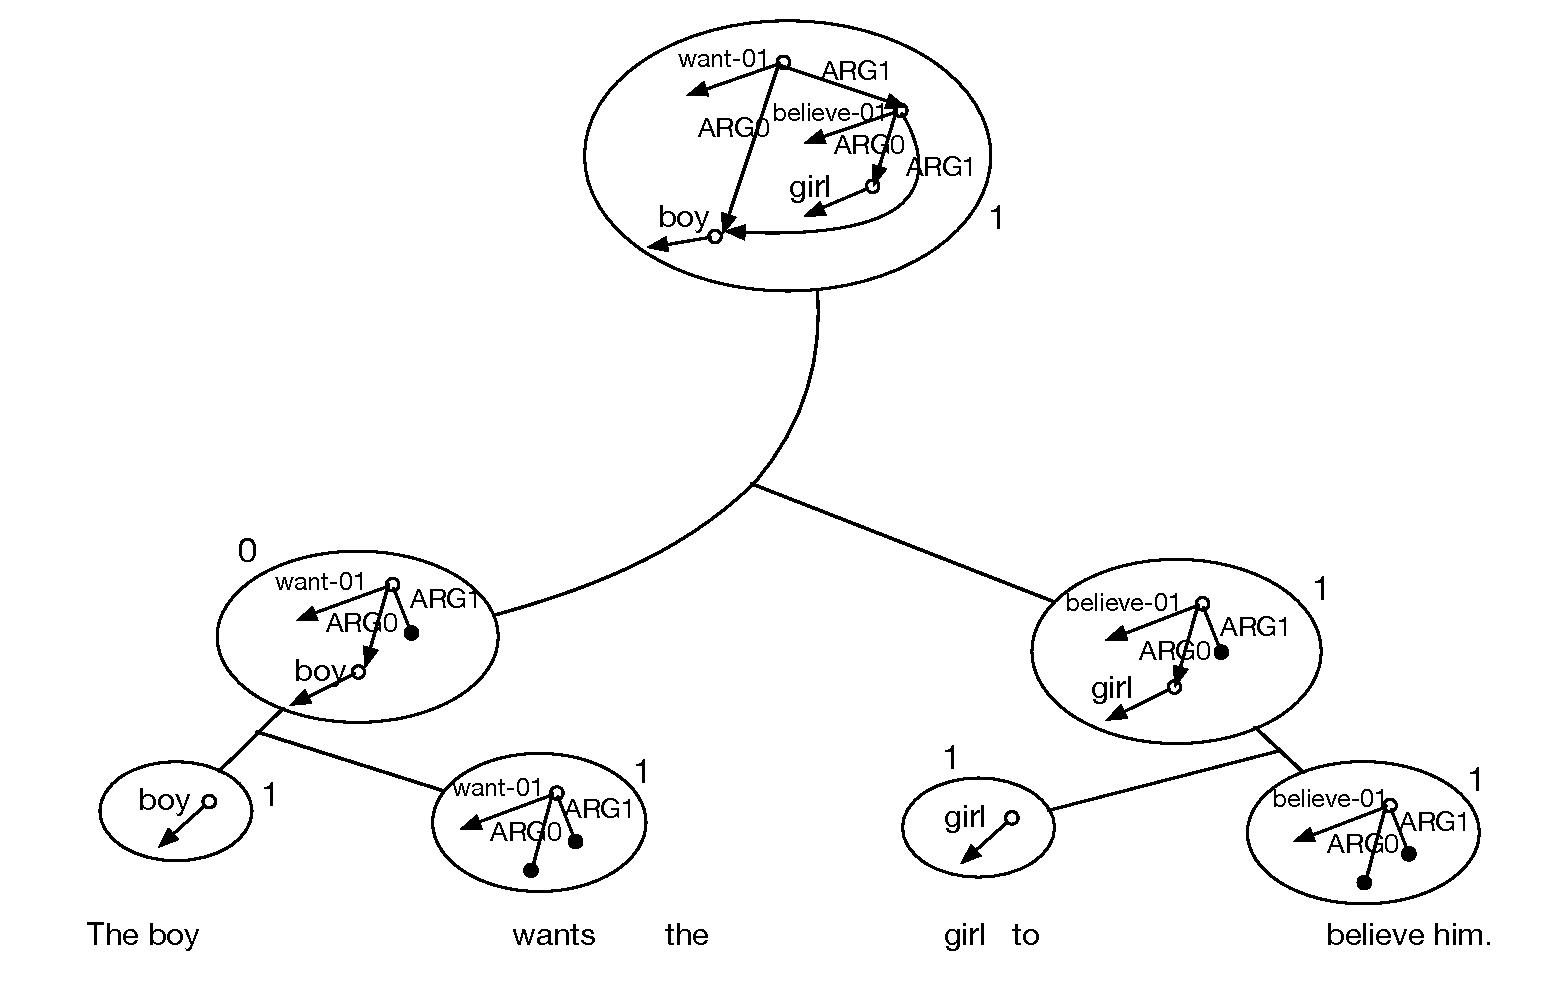
\includegraphics{./Sampled.eps}
%}
%%}
%\caption{The sampled derivation for the (sentence, AMR graph) pair for ``The boy wants the girl to believe him"}
%\label{fig:sampled-example}
%\end{center}
%\end{figure}
%
%Let all the edge variables form the random vector $Y$ and all the cut variables form the random vector $Z$. Given an assignment $y$ to the edge variables and assignment $z$ to the cut variables, our desired distribution is proportional to the product of weights of the rules specified by the assignment:
%\begin{equation}\label{eq:tsg}
% P_t(Y=y, Z=z) \propto \prod_{r \in \tau(y, z)} w(r) 
%\end{equation}
%where $\tau(y, z)$ is the set of rules identified by the assignment and $w(r)$ is the weight for each individual rule. We use a generative model based on a Dirichlet Process (DP) defined over composed rules. We draw a distribution $G$ over rules from a DP, and then rules from $G$. 
%\begin{align*}
%G\mid \alpha,P_0\sim& Dir(\alpha,P_0)\\
%r\mid G\sim& G
%\end{align*}
%
%We define two rules to have the same {\bf rule type} if they have the same string and hypergraph
%representation (including order of external nodes) on the r.h.s..%\footnote{We use special technique of hashing the edge labels, depth of nodes and external nodes sequence to decide the type of graph}
%For the base distribution $P_0$, we use a uniform distribution where all rules of the same size have equal probability.
%By marginalizing out $G$ we get a simple posterior distribution over rules which can be derived using the Chinese Restaurant Process (CRP). 
%
%
%We define a 
%table of counts $N=\{N_C\}_{C\in I}$ which memorizes different categories of counts in 
%the previous assignments, where $I$
%is an index set for different categories of counts. Each $N_C$ is a vector of counts for category $C$. 
%We have the following probability over rule $r$ given the previous count table $N$:
%\begin{equation}
%P(r_i = r| N) = \frac{N_R(r) + \alpha P_0 (r)}{n + \alpha }
%\end{equation}
%here in the case of DP, $I=\{R\}$, where $R$ is the index for the category of rule counts.%\footnote{Using this denotation, we can also adopt other priors like Pitman-Yor or other process priors as long as they satisfy exchangeability property} $N_R(r)$ is the number of times that rule $r$ has been observed in the previous assignment, $n=\sum_r N_R(r)$ is the total number of rules observed.
%
%We use the {\em top-down} sampling algorithm of \namecite{chung-cl14} which samples cut and edge variables from top down and one at a time.
%% (see Algorithm~\ref{alg:topdown}). 
%For each node $n$, we denote the composed rule type
%that we get when we set the cut of node $n$ to 0 as $r_1$ and the two 
%split rule types that we get when we set the cut to 1 as $r_2, r_3$. We sample the cut value $z_i$ of the 
%current node according to the posterior probability:
%\begin{equation}
%\label{eq:cut}
%%$$
%\resizebox{.88\hsize}{!}{$\displaystyle
%P(z_i = z| N) = 
%\begin{cases} 
%\frac{ P (r_1| N) }{P (r_1|N) + P (r_2| N) P (r_3| N') } &\mbox{if } z = 0 \\ 
%\frac{ P (r_2| N) P (r_3| N') }{P (r_1| N)+ P (r_2| N) P (r_3| N') } &\mbox{otherwise}
%\end{cases}$}
%%$$
%\end{equation}
%where the posterior probability $P(r_i|N)$ is according to a DP, 
%and $N, N'$ are tables of 
%counts. In the case of DP, $N, N'$ differ only in the rule counts of $r_2$, where $N'_R(r_2)= 
%N_R(r_2)+1$.
%
%
%As for edge variables $e_i$, we refer to the set of composed rules turned on below $n$ including the 
%composed rule fragments having $n$ as an internal or root node as $\{r_1,\ldots,r_m\}$. We have the 
%following posterior probability over the edge variable $e_i$:
%\begin{equation}
%\resizebox{.88\hsize}{!}{$\displaystyle
%P(e_i = e| N) \propto \prod_{i=1}^m P(r_i| N^{i-1}) \prod_{v \in \tau(e)\cap \mbox{in}(n)} \mbox{deg}(v)
%$}
%\end{equation}
%where $\mbox{deg}(v)$ is the number of incoming edges for node $v$, 
%$\mbox{in}(n)$ is the set of nodes 
%in all subtrees under $n$, and $\tau(e)$ is the tree specified when we set $e_i = e$. $N^0$ to $N^m$ 
%are tables of counts where $N^0 = N$, $N^i_R(r_i) = N^{i-1}_R(r_i) + 1$ in the case of DP.
%
%
%After we have sampled one SHRG derivation from the forest, we still need to keep track of the place where each nonterminal edge attaches.
%As we have maintained the graph fragment it represents in each node of the forest, we can retrieve the attachment nodes of each hyperedge in the r.h.s.\ by tracing at 
%which graph nodes two fragments fuse with each other. We perform this rule extraction procedure from top-down and maintain the order of attachment nodes of each r.h.s.\
%nonterminal edge.
%When we further rewrite a nonterminal edge, we need to make sure that it keeps the order of the attachment nodes in its parent rule. 
%As for the unaligned words, we just insert all the omitted unaligned words in the
%composition procedure. We also add additional rules including the surrounding 2 unaligned words context to
%make sure there are terminals on the string side.
%
%\subsection{Phrase-to-Graph-Fragment Alignment Extraction}
%Aside from the rules sampled using the MCMC algorithm,
%we also extract a phrase-to-graph-fragment alignment table from the fragment decomposition forest.
%This step can be considered as a mapping of larger phrases made of multiple identified spans (plus unaligned words) to a larger fragments made of multiple concept fragments (plus the way they connect using unaligned edges).
%
%
%Our extraction happens along with the forest construction procedure. In line~\ref{1st} of Algorithm~\ref{alg:forest}
%we extract one rule for each smallest phrase-fragment pairs before and after the unaligned
%edges are attached. We also extract one rule for each newly constructed node after line~\ref{new} 
%if the fragment side of the node is single-rooted.\footnote{Here we will also look at the surrounding 2 unaligned words to fix partial alignment and noise introduced
%by meaningful unaligned words}
%We do not extract rules after line~\ref{2nd} because it
%usually introduces additional noise of meaningful concepts which are unrecognized in the concepts
%identification stage. %For named entities and time expressions that can not be found in
%%our training data, we use the alignment result from the concept identification stage of \namecite{flanigan2014discriminative}.
%\section{Decoding}
%\subsection{Concept identification}
%During the decoding stage, first we need to identify meaningful spans in the sentence and map them to graph fragments on the graph side. Then we use SHRG rules to
%parse each sentence from bottom up and left to right, which is similar to constituent parsing. The recall of the concept identification stage from \namecite{flanigan2014discriminative} is 0.79, which means 21\% of the meaningful concepts are already lost at the beginning of the next stage. 
%
%
%Our strategy is to use lemma and POS tags information after the concept identification stage, we use it to recall some meaningful
%concepts. We find that, except for some special function words, most nouns, verbs and, adjectives
%should be aligned. We use the lemma information to retrieve unaligned words whose morphological form does not appear in our training data. 
%We also use POS tag information to deal with nouns and quantities. Motivated by the fact that AMR makes extensive use of PropBank framesets,
%we look up the argument structure of the verbs from the PropBank. Although the complicated abstraction of AMR
%makes it hard to get the correct concept for each word, the more complete structure can reduce the propagation of errors along the derivation tree.
%
%
%\subsection{AMR graph parsing}\label{sec:decode}
%We use Earley algorithm with cube-pruning \cite{ChiangCL} for the string-to-AMR parsing. 
%For each synchronous rule with $N$ nonterminals on its l.h.s., we build an $N+1$ dimensional cube and generate top $K$ candidates. 
%Out of all the hypotheses generated by all satisfied rules within each span $(i,j)$,we keep at most $K$ candidates for this span.
%Our glue rules will create a pseudo $R/ROOT$ concept and use $ARG$s relations to connect
%disconnected components to make a connected graph.
%%We use glue rule to connect two sub-graphs which a NULL edge.
%
%
%We use the following local features:
%\begin{enumerate}\footnotesize
%    \item StringToGraphProbability: the probability of a hypergraph given the input string
%    \item RuleCount: number of rules used to compose the AMR graph
%    \item RuleEdgeCount: the number of edges in the r.h.s.\ hypergraph 
%    \item EdgeType: the type of the l.h.s.\ nonterminal. For rules with same source side tokens, we prefer rules with smaller edge types.
%    \item AllNonTerminalPunish: one for rules which only have non-terminals on the source side.
%    \item GlueCount: one for glue rules.  
%\end{enumerate}
%As our forest structure is highly binarized, it is hard to capture the \textit{:op}n structure when $n$ is large because we limit the number
%of external nodes to 5. The most common \textit{:op} structure in the AMR annotation is the coordinate structure of items separated by ``;" or separated by ``," along with
%$and$. We add the following two rules:
%\begin{align*}
%    &\resizebox{.8\hsize}{!}{$[X\text{1-1}] -> [X\text{1-1}, 1] ; [X\text{1-1}, 2] ; \cdots ; [X\text{1-1}, n]\ |$}\\
%    &\quad \resizebox{.85\hsize}{!}{$(. \textit{ :a/and :op1 } [X\text{1-1}, 1] \textit{ :op2 } [X\text{1-1}, 2] \cdots \textit{ :op}\text{n}\ [X\text{1-1}, n] )$} \\
%    &\resizebox{.8\hsize}{!}{$[X\text{1-1}] -> [X\text{1-1}, 1] , [X\text{1-1}, 2] , \cdots \textit{ and } [X\text{1-1}, n]\ |$}\\
%    &\quad \resizebox{.85\hsize}{!}{$(. \textit{ :a/and :op1 } [X\text{1-1}, 1] \textit{ :op2 } [X\text{1-1}, 2] \cdots \textit{ :op}\text{n}\ [X\text{1-1}, n] )$} 
%\end{align*}
%where the HRG side is a \textit{:a/and} coordinate structure of \textit{X}1-1s connected with relation \textit{:op}s.
%\section{Experiments}
%We use the same newswire section of LDC2013E117 as \namecite{flanigan2014discriminative}, which consists of 3955 training sentences, 2132 dev sentences and 2132 test sentences. We also use 
%the string-to-graph alignment from \namecite{flanigan2014discriminative} to construct the fragment decomposition forest and 
%to extract the phrase-to-fragment table.
%
%
%In the fragment decomposition forest construction procedure, we have experimented with
%different ways of dealing with the unaligned edges. First we have tried to
%directly use the alignment, and group all unaligned edges going out from the same node as an unaligned fragment. Using this constraint would take a few hours or longer for some sentences.
%The reason for this is because the many number of unaligned edges can connect to each branch of the aligned or unaligned fragments below it. And there is no explicit order of composition with each branch. Another constraint we have tried is to attach all unaligned edges to the head node concept. The problem with this constraint is that
%it is very hard to generalize and introduces a lot of additional redundant relation edges.
%
%
%As for sampling, we initialize all cut variables in the forest as 1 (except for nodes that are marked as $nosample\_cut$, which indicates we initialize it with 0 and keep it fixed) and uniformly sample an incoming edge for each node.
%\begin{table}
%\centering
%\scalebox{0.8}{
%\begin{tabular}{|l|l|l|l|} \hline
%                & Precision             & Recall       & F-score  \\ \hline 
%    Concept id only &     0.37           &   0.53   & 0.44     \\ \hline
%    + MCMC&  0.57              &  0.53    &  0.55    \\ \hline
%    + MCMC + phrase table &   0.60             &  0.54    &  0.57    \\ \hline
%    + All             & 0.59   &  0.58 & 0.58 \\ \hline
%
%\end{tabular}}
%\caption{Comparisons of different strategies of extracting lexical rules on dev.}
%\label{tab:smatch}
%\end{table}
%We evaluate the performance of our SHRG-based parser using Smatch v1.0 \cite{cai2013smatch}, which
%evaluates the precision, recall and $F1$ of the concepts and relations all together.
%Table~\ref{tab:smatch} shows the dev results of our sampled grammar using different lexical rules
%that maps substrings to graph fragments. Concept id only is the result of using the concepts identified by \namecite{flanigan2014discriminative}. From second line, we replace the concept identification result with the lexical rules we have extracted from the training data (except for named entities and time expressions). 
%+MCMC shows the result using additional alignments identified using our sampling approach. We can see that
%using the phrase to graph fragment alignment learned from our training data can significantly improve the smatch.
%We have also tried extracting all phrase-to-fragment alignments of length 6 on the string side 
%from our constructed forest. We can see that using this alignment table further improves the smatch score.
%This is because the larger phrase-fragment pairs can make better use of the dependency information
%between continuous concepts. The improvement is not much in comparison with MCMC, this is perhaps 
%MCMC can also learn some meaning blocks that frequently appear together.
%As the dataset is relatively small, so there are a lot of meaningful concepts that are not aligned. We use lemma as a backoff strategy to find
%the alignment for the unaligned words. We have also used the POS tag information to retrieve some unaligned nouns and a PropBank dictionary to 
%retrieve the argument structure of the first sense of the verbs. +All
%shows the result after using lemma, POS tag and PropBank information, we can see that fixing the alignment can improve the recall, but the precision does not change much. 
%\begin{table}
%\centering
%\scalebox{0.8}{
%\begin{tabular}{|l|l|l|l|} \hline
%                & Precision             & Recall       & F-score  \\ \hline 
%    JAMR      &  0.67              &  0.58    & 0.62     \\ \hline
%    Wang et al. & 0.64 & 0.62 & 0.63 \\ \hline
%    Our approach          &   0.59           & 0.57     & 0.58          \\ \hline
%\end{tabular}}
%\caption{Comparisons of smatch score results}
%\label{tab:tsmatch}
%\end{table}
%
%Table~\ref{tab:tsmatch} shows our result on test data. JAMR is the baseline result from \namecite{flanigan2014discriminative}. \namecite{wang-xue-pradhan:2015:NAACL-HLT} shows the current state-of-art for string-to-AMR parsing.
%Without the dependency parse information and complex global features, our SHRG-based approach can already achieve competitive results in comparison with these two algorithms.

\section{Forced decoding}
The generative decoding model has a few limitations: 1. the features are very simple and no global feature is included. 2. All the weights of the features are
set by hand, which suffers from the limit of huge space of combination of the weights.
One way to deal with these limitations is to use a feature-rich discriminative model. The training data is used to extract the SHRG, more specifically
rules and the count for each rule. However, the structural information of the derivation forest is not used. Using a discriminative model which
learns to search within the forest structure would make use of more structural information in our training data.


\namecite{yu-EtAl:2013:EMNLP} have proposed a structured perceptron algorithm that learns to search for derivations that generate the whole or prefixes of the 
target reference sentences for phrase-based machine translation. Beam search is used to reduce the intractable search space and each bin $B_i$ maintain a K-best list of hypotheses that covers $i$ words
on the source side. A search error happens for a certain hypothesis $d$ when its target side $e(d)$ is not a prefix of the reference $y$.

\subsection{Forced decoding for AMR parsing}
In our AMR parsing scenario, we have a derivation forest representing possible ways to compose sentence-AMR pairs. Let $<x, y>$ be a sentence-AMR pair in the training data. We can 
compare the AMR graph side to the target side sentence and each hypothesis $d$ contains a span-subgraph pair derived from a series of rule applications:
$$d = r_1 \circ r_2 \circ \cdots \circ r_{|d|}$$
where each $r_i$ is a SHRG rule and $d=(e(d), g(d))$ is a (partial) derivation whose source side $e(d)=(x_i, \cdots , x_j)$ is a span which covers 
positions $[i, j]$ and whose target side is a subgraph $g(d)$ generated so far. 


We maintain the a bin $B_{ij}$ for each span $[i, j]$. Let $sub(y)$ be all the subgraphs
of target side AMR $y$ and $good_{ij} (x, y)$ be set of partial $y$-good derivations whose graph side is a subgraph of the reference AMR graph $y$
and the sentence side covers span $[i, j]$:
$$good_{ij}(x, y)\triangleq \{d \in D(x) | g(d) \in sub(y), e(d)=(x_i, \cdots , x_j)\}$$

Conversely, we define $y$-bad partial derivations $bad_{ij}(x,y)$ as follows:
$$bad_{ij}(x, y)\triangleq \{d \in D(x) | g(d) \notin sub(y), e(d)=(x_i, \cdots , x_j)\}$$

The search using Earley algorithm proceeds as follows: use the \textit{scan} and \textit{complete} operation to find items that covers source span $[i, j]$. 
The cost for each item is scored as: 
$${\bf w} \cdot {\bf \Phi}(x, d, i, j)$$
where $d$ is the partial derivation constructed so far. $\Phi$ is the features extracted within span $[i, j]$ and the partial derivation $d$. We keep two separate
grammars to derive $good_{ij}(x, y)$ and $bad_{ij}(x, y)$. The $good_{ij}(x, y)$ is constructed by searching along the constructed forest, that is, follow the supervision of
the composition of the sentence-AMR pair and therefore always derives a partial $y$-good derivations. $bad_{ij}(x, y)$ is constructed by searching through the whole grammar, which tries to find the derivation that has the greatest
global score. Assume we have $K$ items at each bin, we gradually build up each bin using recursion:
$$B_0 = \{ \emptyset \}$$
$$B_{ij} = \textbf{top}^K (good_{ij}(x,y)) \cap \textbf{top}^K (bad_{ij}(x,y))$$
where $\textbf{top}^K$ is an operator which computes the top $K$ items of a stack according to the scoring function.
\subsection{Parameter update}
The perceptron works by adjusting the weights whenever search error happens and different variations of the perceptron algorithm make update
at different points. The standard perceptron algorithm works by decoding the whole sentence first and update if the predication for the whole
sentence does not match the reference. This update has the problem that in cases where search error happens at a very early step and there is
no $y$-good item left in the bin. There is little point in continuing the search and update the parameters afterwards.


Early update is a special case of violation-fixing perceptron which stops decoding whenever the gold derivation falls off the beam. It makes update on the partial derivation so far and 
move on to the next training example when the update finishes. As we don't actually have the gold derivation, we replace it with
the item in $good_{ij}(x,y)$ that has the largest score.
$$d_{ij}^{+} \equiv {\bf \argmax}_{d\in good_{ij}(x,y)} {\bf w}\cdot \Phi(x, d, i, j)$$
$$d_{ij}^{-} \equiv {\bf \argmax}_{d\in bad_{ij}(x,y)} {\bf w}\cdot \Phi(x, d, i, j)$$
$${\bf w} \leftarrow {\bf w} + \triangle \Phi(x, d_{ij}^{+}, d_{ij}^{-}, i, j)$$
where $\triangle \Phi(x, d, d', i, j) \equiv \Phi(x, d, i, j) - \Phi(x, d', i, j)$ is the notation for the difference of feature vectors.


In practice, there are exponentially many $y$-good derivations for each sentence-AMR pair and our goal is to make sure the $y$-good derivation would succeed in the end. 
It is possible that in a certain span $[i,j]$ all $y$-good derivations fall off the bin, but search can still succeed from other spans.
Therefore, we will continue the search through all possible spans until we reach the condition that there is no hope of finding another 
$y$-good derivation.


Another way of doing parameter update is to use \textit{max-violation} proposed by Huang et al. (2012). The basic idea is to update at the
point where the mistake is the biggest. More specifically, the update step is:
$$(ij)^{*} \equiv {\argmin}_{ij} {\bf w} \cdot \triangle \Phi(x, d_{ij}^{+}, d_{ij}^{-}, i, j)$$
$${\bf w} \leftarrow {\bf w} + \triangle \Phi(x, d_{(ij)^*}^{+}, d_{(ij)^*}^{-}, i, j)$$
%\begin{algorithm}[t]
%\small
%\caption{Forced Earley decoding for AMR parsing}
%\begin{algorithmic}[1]
%\STATE{Initialize $B_0 = \{\emptyset \}$}
%\FOR{$i = 1,\cdots , n$:} 
%    \FOR{$j = 1,\cdots , n$:}
%        \STATE{Scan} 
%        \STATE{$B_{ij} = $}
%    \ENDFOR
%\ENDFOR
%\end{algorithmic}
%\label{alg:gibbs}
%\end{algorithm}
\section{Conclusion}
We have presented an MCMC algorithm for sampling SCFG rules from derivation forests constructed from aligned sentence-AMR pairs.
With the extracted grammar, we used Earley algorithm with cubing pruning to decode each sentence. To overcome the limitations of
simple local features and the hand-tuned weights for each feature, we propose a feature-rich discriminative model using forced decoding to
include rich global features and adjust the weights using perceptron update.
